Compared to the initial version of the SG-t-SNE-Pi algorithm in c/c++, the pure julia version of the algorithm 
is lacking. After around 8 threads we encounter diminishing returns. We reached a point where we exceeded 
the physical threads enough to gain minimal to no boost in performance. If we had more physical threads 
we could benefit from assigning more Julia threads to the program. However since we want it to be able to 
run on various hardware and the Julia wrapper highlighted significantly better performance on the same 
hardware, the pure julia implementation methods would have to change. The following profiling proves that 
we succeeded in minimizing the negative impact of attraction\_force:
\begin{figure}[H]
    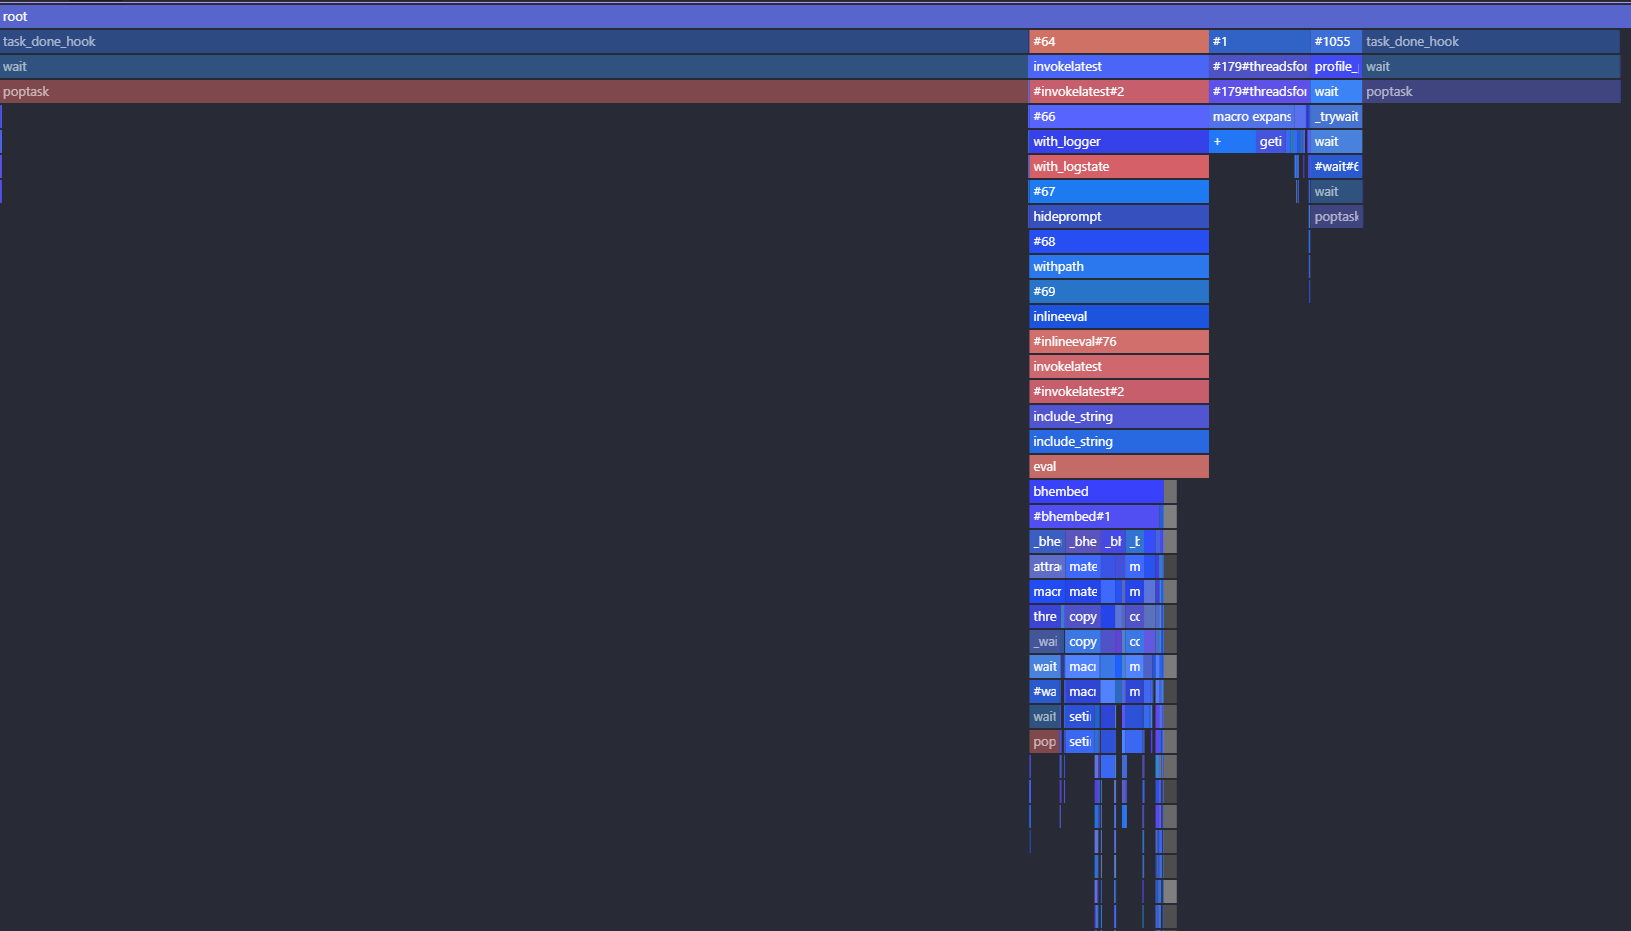
\includegraphics[width=0.5\textwidth]{media/bhembedProfiling.png}
    \caption{Profiling the best pure Julia version}
\end{figure}
with a profiling time of 147 seconds. \\

As we see:
\begin{itemize}
    \item function bhembed, 8\%
    \item In embed: z = \_embed!(), 8\%
    \item In attraction\_force\_symm!(): 
    \begin{minted}[breaklines,escapeinside=||,
                mathescape=true, 
                linenos, 
                numbersep=3pt, 
                gobble=2, 
                frame=lines, 
                fontsize=\small, 
                framesep=2mm]{julia}
        Fattr[j,l] += pq * (Yj[l] - Yi[l]) # 5%
    \end{minted}
\end{itemize}
with everything else being below 2\%. \\

To conclude, it seems that the key to advancing the sgtsnepi pure julia project most likely lies in 
understanding the last profiling results.